% Native editable composition from verified, unchanged IDE images.
\begin{figure}[htbp]
  \centering
  \sbox0{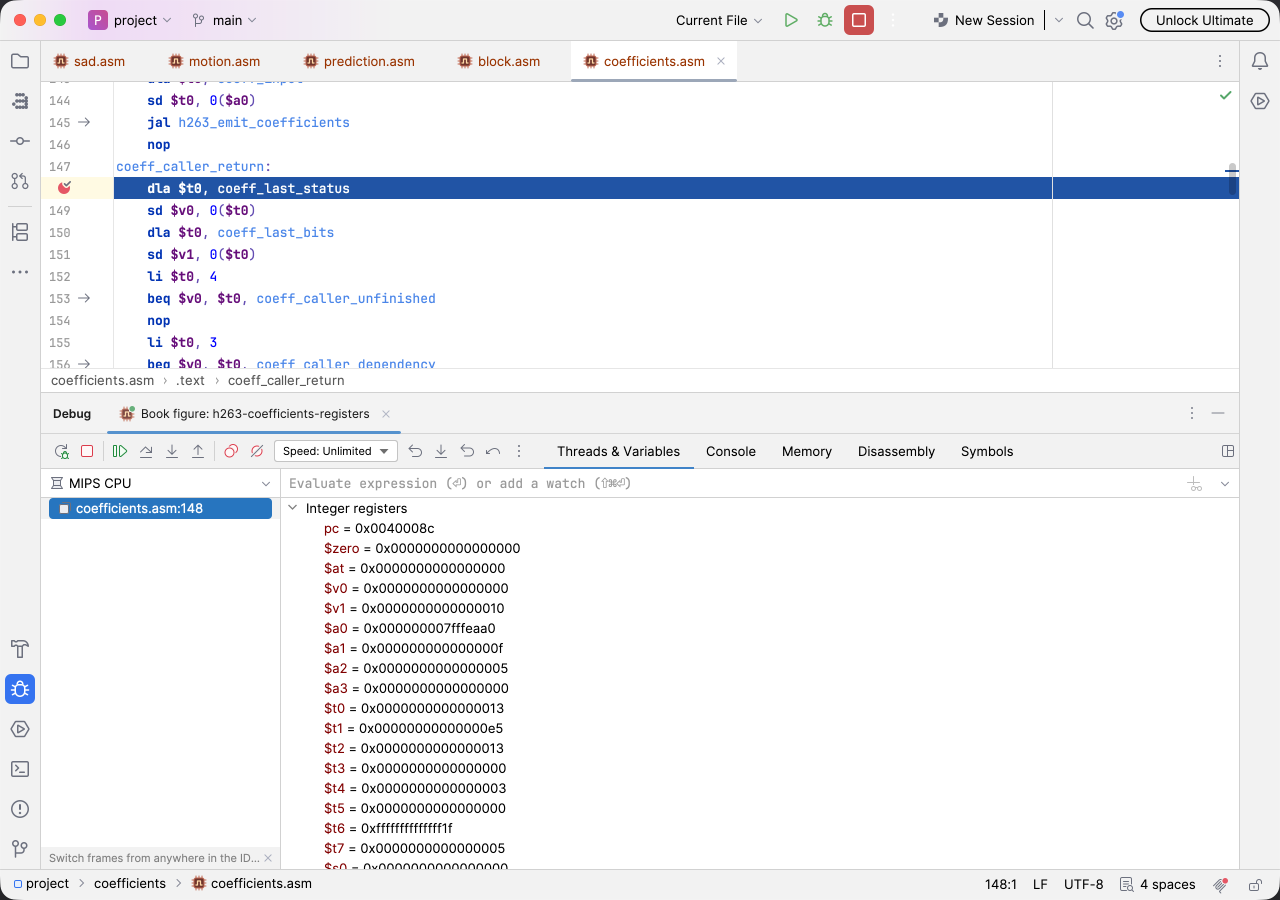
\includegraphics[artifact]{packages/035-h263/captures/h263-coefficient-bits/registers.png}}
  \sbox2{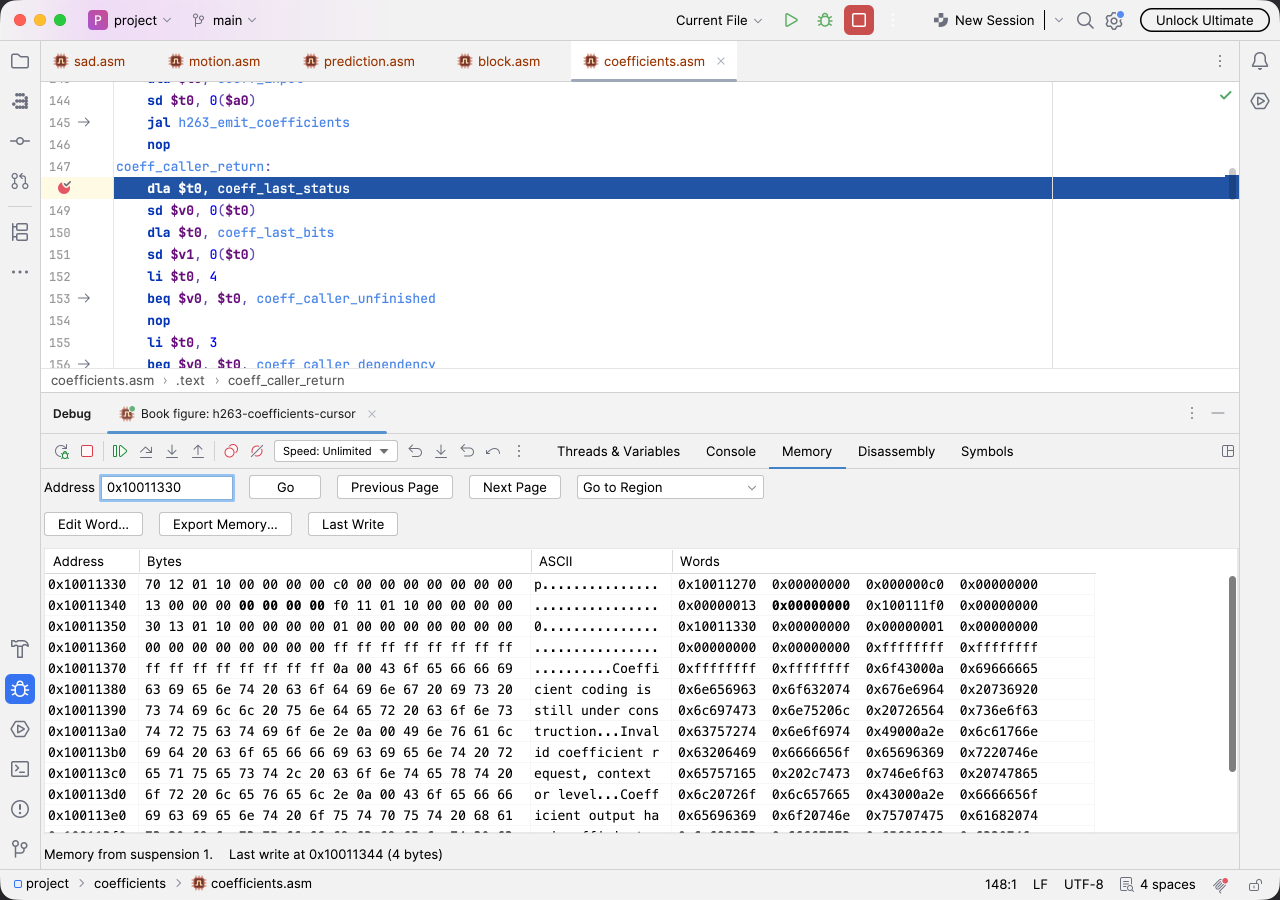
\includegraphics[artifact]{packages/035-h263/captures/h263-coefficient-bits/cursor.png}}
  \sbox4{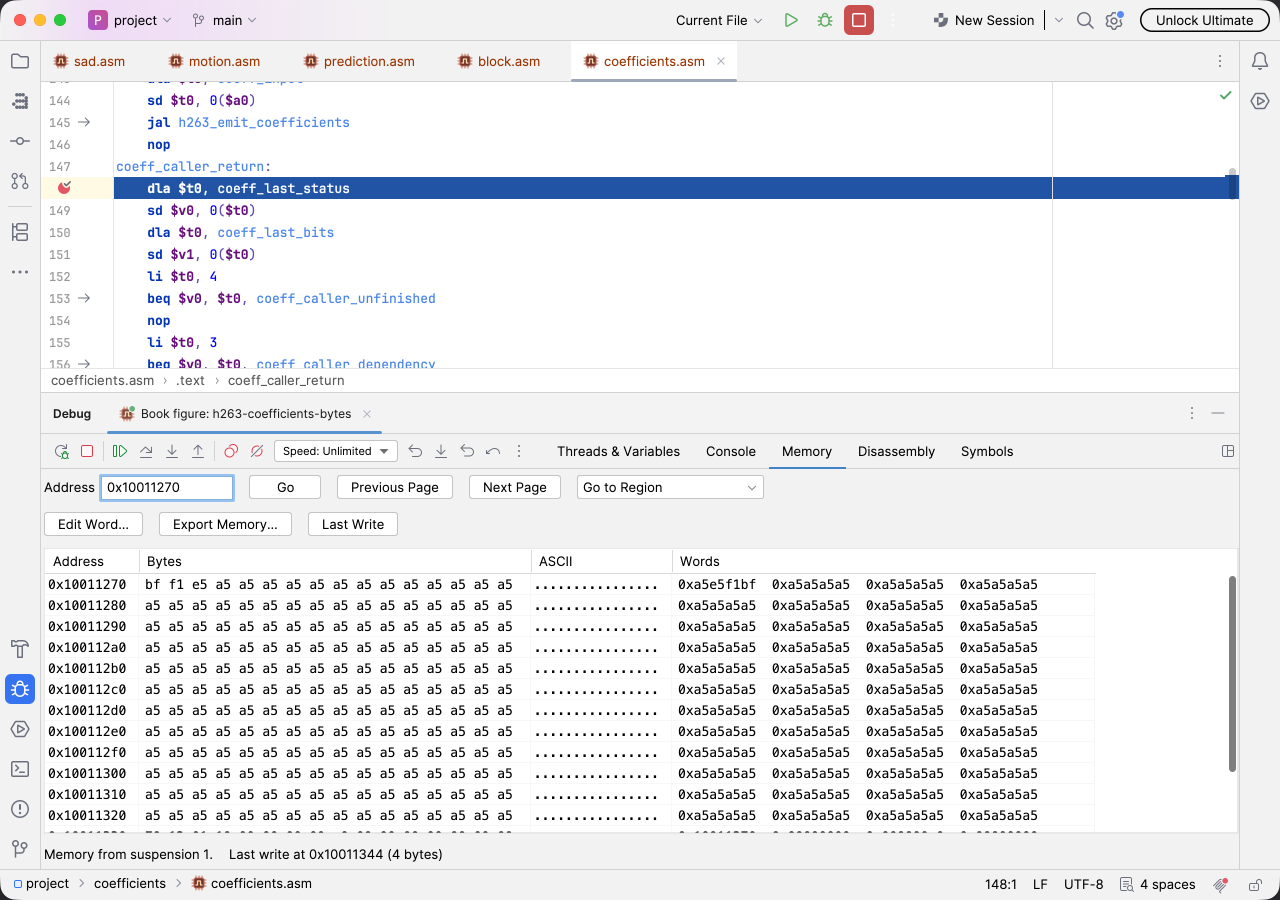
\includegraphics[artifact]{packages/035-h263/captures/h263-coefficient-bits/bytes.png}}
  \edef\MARScoefficientssourceLeft{\the\dimexpr0.036718750\wd0\relax}
  \edef\MARScoefficientssourceBottom{\the\dimexpr0.774444444\ht0\relax}
  \edef\MARScoefficientssourceRight{\the\dimexpr0.611718750\wd0\relax}
  \edef\MARScoefficientssourceTop{\the\dimexpr0.170000000\ht0\relax}
  \edef\MARScoefficientscursorLeft{\the\dimexpr0.108593750\wd2\relax}
  \edef\MARScoefficientscursorBottom{\the\dimexpr0.312222222\ht2\relax}
  \edef\MARScoefficientscursorRight{\the\dimexpr0.585156250\wd2\relax}
  \edef\MARScoefficientscursorTop{\the\dimexpr0.634444444\ht2\relax}
  \edef\MARScoefficientsbytesLeft{\the\dimexpr0.108593750\wd4\relax}
  \edef\MARScoefficientsbytesBottom{\the\dimexpr0.335555556\ht4\relax}
  \edef\MARScoefficientsbytesRight{\the\dimexpr0.585156250\wd4\relax}
  \edef\MARScoefficientsbytesTop{\the\dimexpr0.634444444\ht4\relax}
  \edef\MARScoefficientsreturnsLeft{\the\dimexpr0.246093750\wd0\relax}
  \edef\MARScoefficientsreturnsBottom{\the\dimexpr0.310000000\ht0\relax}
  \edef\MARScoefficientsreturnsRight{\the\dimexpr0.596875000\wd0\relax}
  \edef\MARScoefficientsreturnsTop{\the\dimexpr0.638888889\ht0\relax}
  \begin{tikzpicture}[alt={Four annotated details at coeff_caller_return. The output starts bf f1 e5 then unchanged a5 bytes. Little-endian context bytes describe output pointer 10011270, capacity c0 or 192 bytes and cursor 13 or 19 bits. The context begins at the first displayed byte; the final displayed doubleword belongs to the following request. Return v0 is zero and v1 is 10 or sixteen appended bits. The highlighted dla precedes the caller stores.}]
    \node[anchor=north west,inner sep=0,font=\small\bfseries] (source-title) at (6mm,0) {Completed coefficient coding};
    \node[anchor=north west,inner sep=0] (source) at ([yshift=-1mm]source-title.south west) {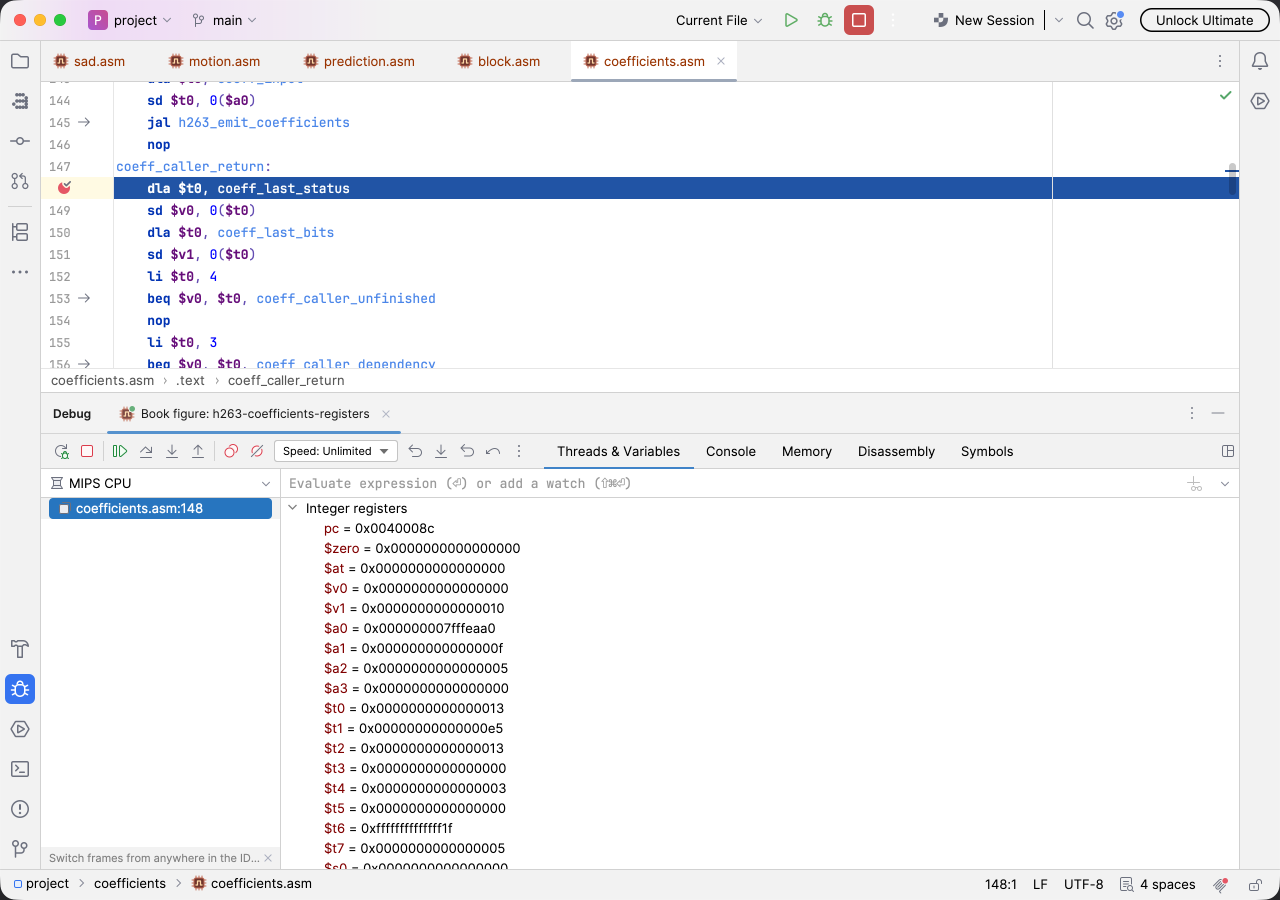
\includegraphics[width=0.7\linewidth,artifact,trim={\MARScoefficientssourceLeft{} \MARScoefficientssourceBottom{} \MARScoefficientssourceRight{} \MARScoefficientssourceTop{}},clip]{packages/035-h263/captures/h263-coefficient-bits/registers.png}};
    \begin{scope}[shift={(source.south west)},x={($(source.south east)-(source.south west)$)},y={($(source.north west)-(source.south west)$)}]
      \draw[black,line width=0.7pt] (0.153333333,0.080000000) rectangle (0.673333333,0.520000000);
      \node[draw=black,fill=white,circle,inner sep=1.5pt,font=\footnotesize] at ($(0.153333333,0.520000000)+(-3mm,0)$) {1};
    \end{scope}
    \node[anchor=north west,inner sep=0,font=\small\bfseries] (cursor-title) at ([yshift=-2mm]source.south west) {Context bytes including retained capacity};
    \node[anchor=north west,inner sep=0] (cursor) at ([yshift=-1mm]cursor-title.south west) {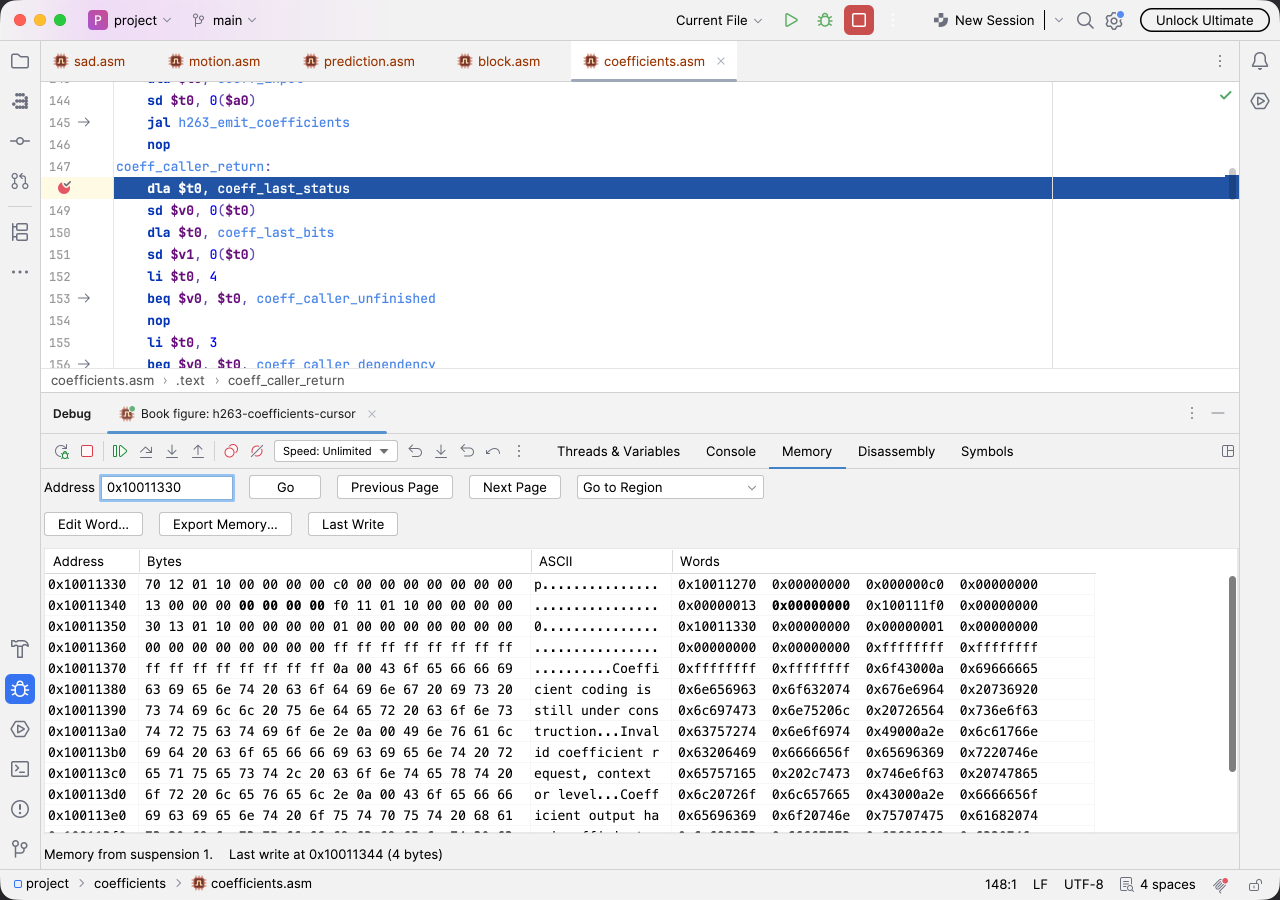
\includegraphics[width=0.84\linewidth,artifact,trim={\MARScoefficientscursorLeft{} \MARScoefficientscursorBottom{} \MARScoefficientscursorRight{} \MARScoefficientscursorTop{}},clip]{packages/035-h263/captures/h263-coefficient-bits/cursor.png}};
    \begin{scope}[shift={(cursor.south west)},x={($(cursor.south east)-(cursor.south west)$)},y={($(cursor.north west)-(cursor.south west)$)}]
      \draw[black,line width=0.7pt] (0.000000000,0.062500000) rectangle (1.000000000,0.937500000);
      \node[draw=black,fill=white,circle,inner sep=1.5pt,font=\footnotesize] at ($(0.000000000,0.937500000)+(-3mm,0)$) {2};
    \end{scope}
    \node[anchor=north west,inner sep=0,font=\small\bfseries] (bytes-title) at ([yshift=-2mm]cursor.south west) {Touched output bytes and retained suffix};
    \node[anchor=north west,inner sep=0] (bytes) at ([yshift=-1mm]bytes-title.south west) {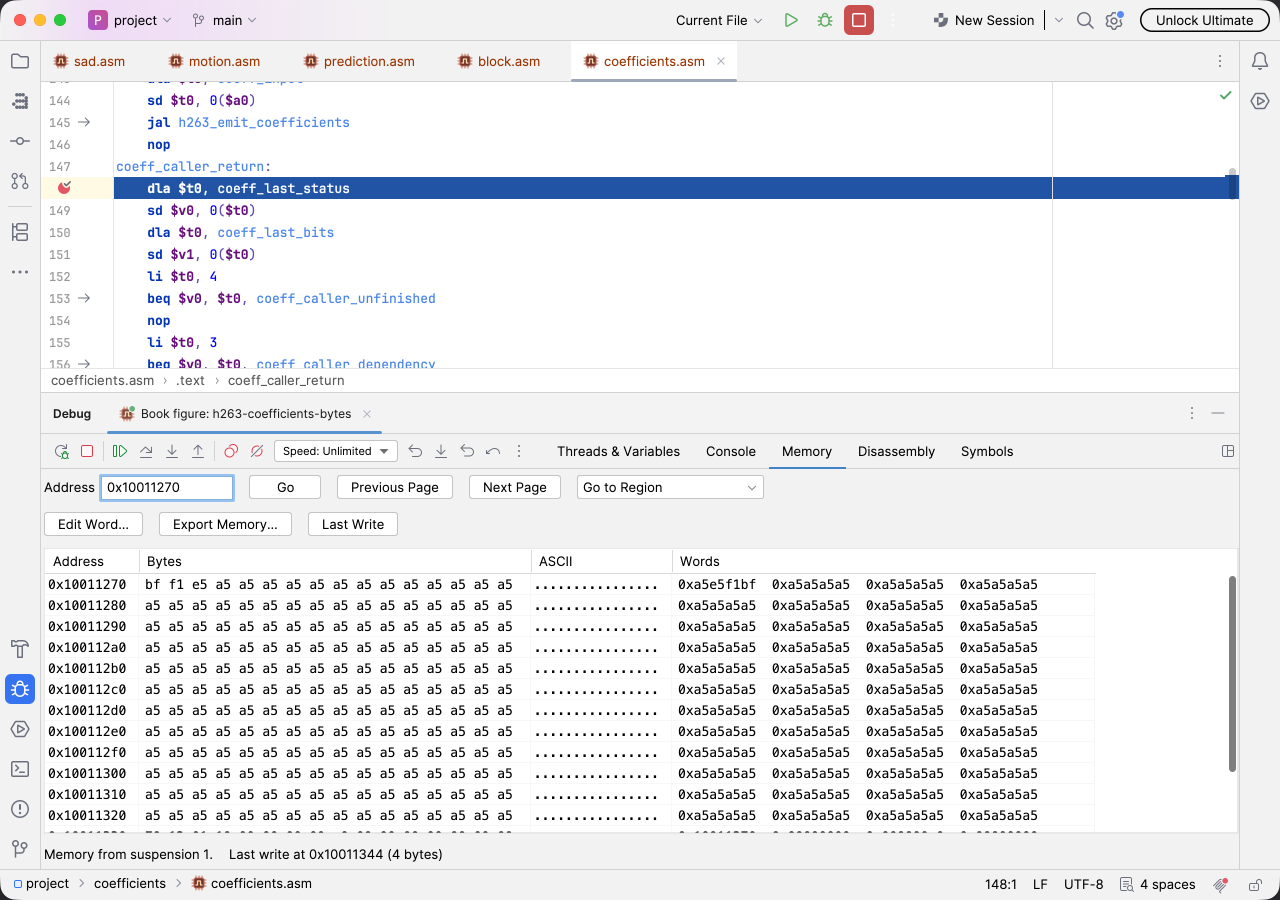
\includegraphics[width=0.84\linewidth,artifact,trim={\MARScoefficientsbytesLeft{} \MARScoefficientsbytesBottom{} \MARScoefficientsbytesRight{} \MARScoefficientsbytesTop{}},clip]{packages/035-h263/captures/h263-coefficient-bits/bytes.png}};
    \begin{scope}[shift={(bytes.south west)},x={($(bytes.south east)-(bytes.south west)$)},y={($(bytes.north west)-(bytes.south west)$)}]
      \draw[black,line width=0.7pt] (0.000000000,0.111111111) rectangle (1.000000000,0.888888889);
      \node[draw=black,fill=white,circle,inner sep=1.5pt,font=\footnotesize] at ($(0.000000000,0.888888889)+(-3mm,0)$) {3};
    \end{scope}
    \node[anchor=north west,inner sep=0,font=\small\bfseries] (returns-title) at ([yshift=-2mm]bytes.south west) {Successful call and appended bit count};
    \node[anchor=north west,inner sep=0] (returns) at ([yshift=-1mm]returns-title.south west) {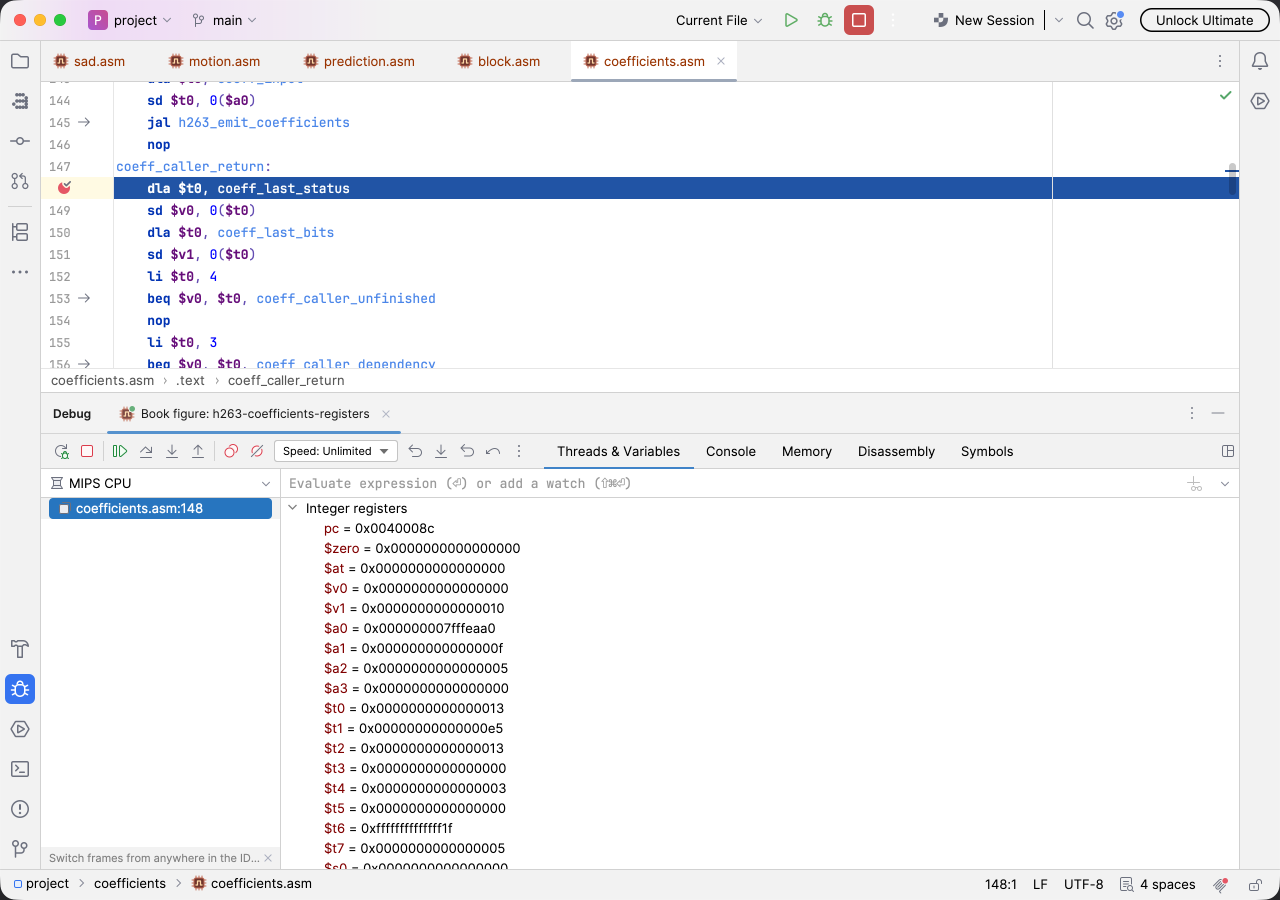
\includegraphics[width=0.5\linewidth,artifact,trim={\MARScoefficientsreturnsLeft{} \MARScoefficientsreturnsBottom{} \MARScoefficientsreturnsRight{} \MARScoefficientsreturnsTop{}},clip]{packages/035-h263/captures/h263-coefficient-bits/registers.png}};
    \begin{scope}[shift={(returns.south west)},x={($(returns.south east)-(returns.south west)$)},y={($(returns.north west)-(returns.south west)$)}]
      \draw[black,line width=0.7pt] (0.029850746,0.065217391) rectangle (0.970149254,0.934782609);
      \node[draw=black,fill=white,circle,inner sep=1.5pt,font=\footnotesize] at ($(0.029850746,0.934782609)+(-3mm,0)$) {4};
    \end{scope}
  \end{tikzpicture}
  \par\smallskip
  \begin{minipage}{\linewidth}
    \small
    \begin{enumerate}
      \item The worked INTRA block uses DC code 255 and two nonzero AC levels. Its compact payload is 16 bits. The routine has returned before the caller saves the status.
      \item The context begins at the first displayed byte. Read eight-byte fields: output pointer, capacity \texttt{0xc0}=192 bytes and used count \texttt{0x13}=19 bits. The last eight bytes shown belong to the following request.
      \item The three touched bytes are \texttt{bf f1 e5}. Writing begins after the first three bits and ends before the last five bits of that third byte. Those surrounding bits retain their original \texttt{a5} pattern; later bytes remain \texttt{a5}. The independent bit model checks the complete buffer.
      \item \texttt{\$v0}=0 and \texttt{\$v1}=\texttt{0x10}=16. The return counts newly appended bits. The context cursor includes the three bits that were already present, giving $3+16=19$.
    \end{enumerate}
  \end{minipage}
  \caption{A compact INTRA coefficient payload appended at bit offset three. Three Debug launches show the same successful call.}
  \label{fig:h263-coefficient-bits}
\end{figure}
